\section{Results}

To demonstrate the usefulness of the enhancements to VTK enabling scientific visualization, and to test various use cases, we have implemented three kinds of applications for the \texttt{vtkRenderWindow} approach: GeometryViewer, VolumeViewer, and MooseViewer using VRUI as the VR toolkit, and one simple example using \texttt{vtkOpenVR}. As the name suggests, the GeometryViewer enables end-users to load geometry files from the disk, the VolumeViewer renders a structured dataset using VTK's GPU-based volume rendering technique, and MooseViewer renders a multi-block unstructured dataset as geometry or volume depending on the end-user's interactive selections. Details on each of these applications or examples with screen captures are provided in the next few sub-sections. 

\subsection{Immersive Environments}

A variety of immersive environment exists from head-mounted displays (HMD) to low cost IQ station~\cite{Sherman:2010} and even four or six sided CAVEs. Immersive applications need to support a large number of immersive environments, as each has their strength and applicability in real world scenarios. We have tested our work in following virtual environments: 

\begin{compactitem}
\item A four-sided CAVE,
\item A low cost IQ station, and 
\item A HTC VIVE.
\end{compactitem}

In the first two cases, the \texttt{vtkRenderWindow} module was used with the Vrui VR toolkit provided the configuration necessary to run the application. For the HTC VIVE, we leveraged \texttt{vtkOpenVR}. 

\subsection{VRUI Implementation}

The task of a VR toolkit is to shield an application developer from the particular configuration of an immersive environment, such that applications can be developed quickly and in a portable and scalable fashion. Three important parts of this overarching goal are: encapsulation of the display environment; encapsulation of the distribution environment; and encapsulation of the input device environment.

The Vrui VR toolkit aims to support fully scalable and portable applications that run on a range of immersive environments starting from a laptop with a touchpad, over desktop environments with special input devices such as space balls, to full-blown immersive VR environments ranging from a single-screen workbench to a multi-screen tiled display wall or CAVE. Applications using the Vrui VR toolkit are written without a particular input environment in mind, and Vrui-enabled immersive environments are configured to map the available displays and input devices to the application such that they appear to be written natively for the environment. For example, a Vrui application running on the desktop should be as usable and intuitive as any 3D application written specifically for the desktop.

We developed some example applications that serve as validation of the said work. There is an example within the VTK source tree for \texttt{vtkRenderingExternal} module that renders a VTK sphere in a GLUT window. Three advanced applications are also developed that illustrate VTK rendering within a Vrui created OpenGL context. These applications exhibit varying capabilities of the VTK infrastructure leveraged by the \texttt{vtkRenderingExternal} module. 

\subsubsection{GeometryViewer}

\begin{figure}[h!]
 \centering
 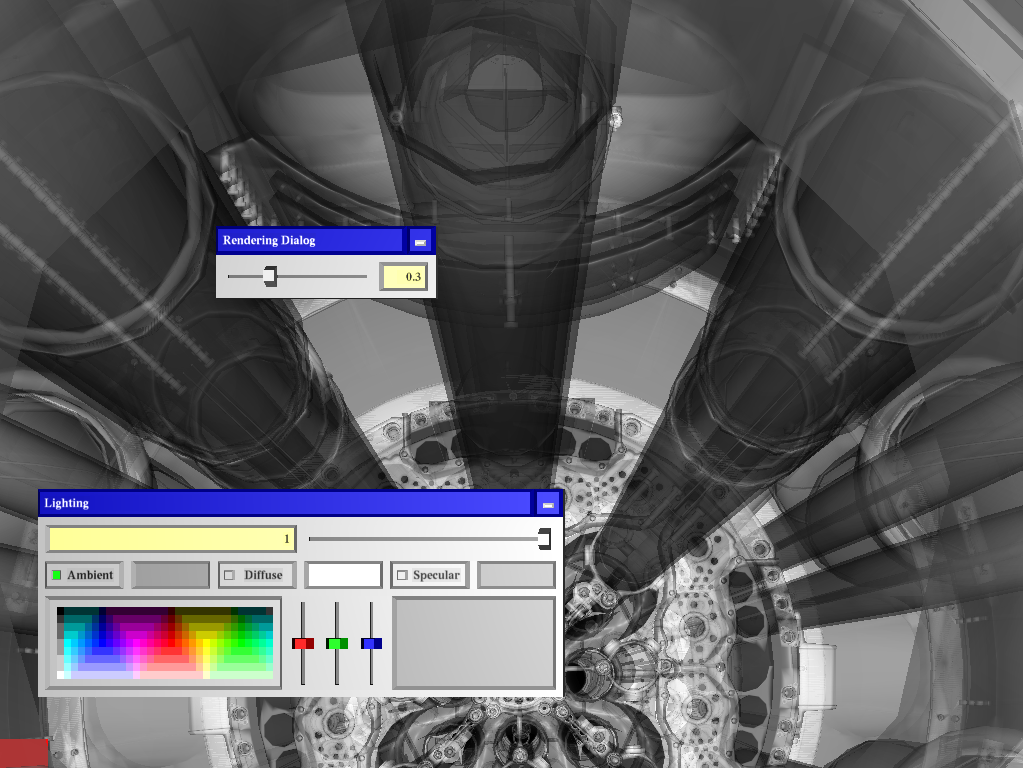
\includegraphics[width=3.5in]{images/vessel.png}
 \caption{The geometry represents Idaho' Nation Laboratory's advanced test reactor (ATR) reactor core, and is used to virtually understand maintenance processes in this extreme environment}
 \label{fig:vessel}
\end{figure}

GeometryViewer~\cite{GeometryViewer} reads in and renders a Wavefront (.obj) file that defines geometry. The file is read using the \texttt{vtkOBJFileReader} that creates \texttt{vtkPolyData} from the geometry. The \texttt{vtkPolyData} is then mapped using VTK's polydata rendering pipeline as a \texttt{vtkActor}. The main menu of the application allows the user to center the geometry to the screen as well as change its representation. The \textit{Center Display} button calculates the transformation from the current camera position and direction to the center position. The \textit{Rendering Options} sub-menu allows the end-user to change the opacity of the \textit{vtkActor}, leveraging our work on dual depth-peeling, as well as its representation to either points, wireframe or surface. In addition to VTK level modifications, the application has support for OpenGL level widgets (e.g. \texttt{glClipPlane}). This shows that native OpenGL operations can also be interactively performed when using the VTK rendering pipeline.

In Figure~\ref{fig:vessel}, we show Vrui's user interface (UI) showing rendering options dialogue allowing us to adjust the transparency of the ATR reactor core. In addition, we used Vrui's UI to build an interface into the lighting color.

\subsubsection{VolumeViewer}

\begin{figure}[h!]
 \centering
 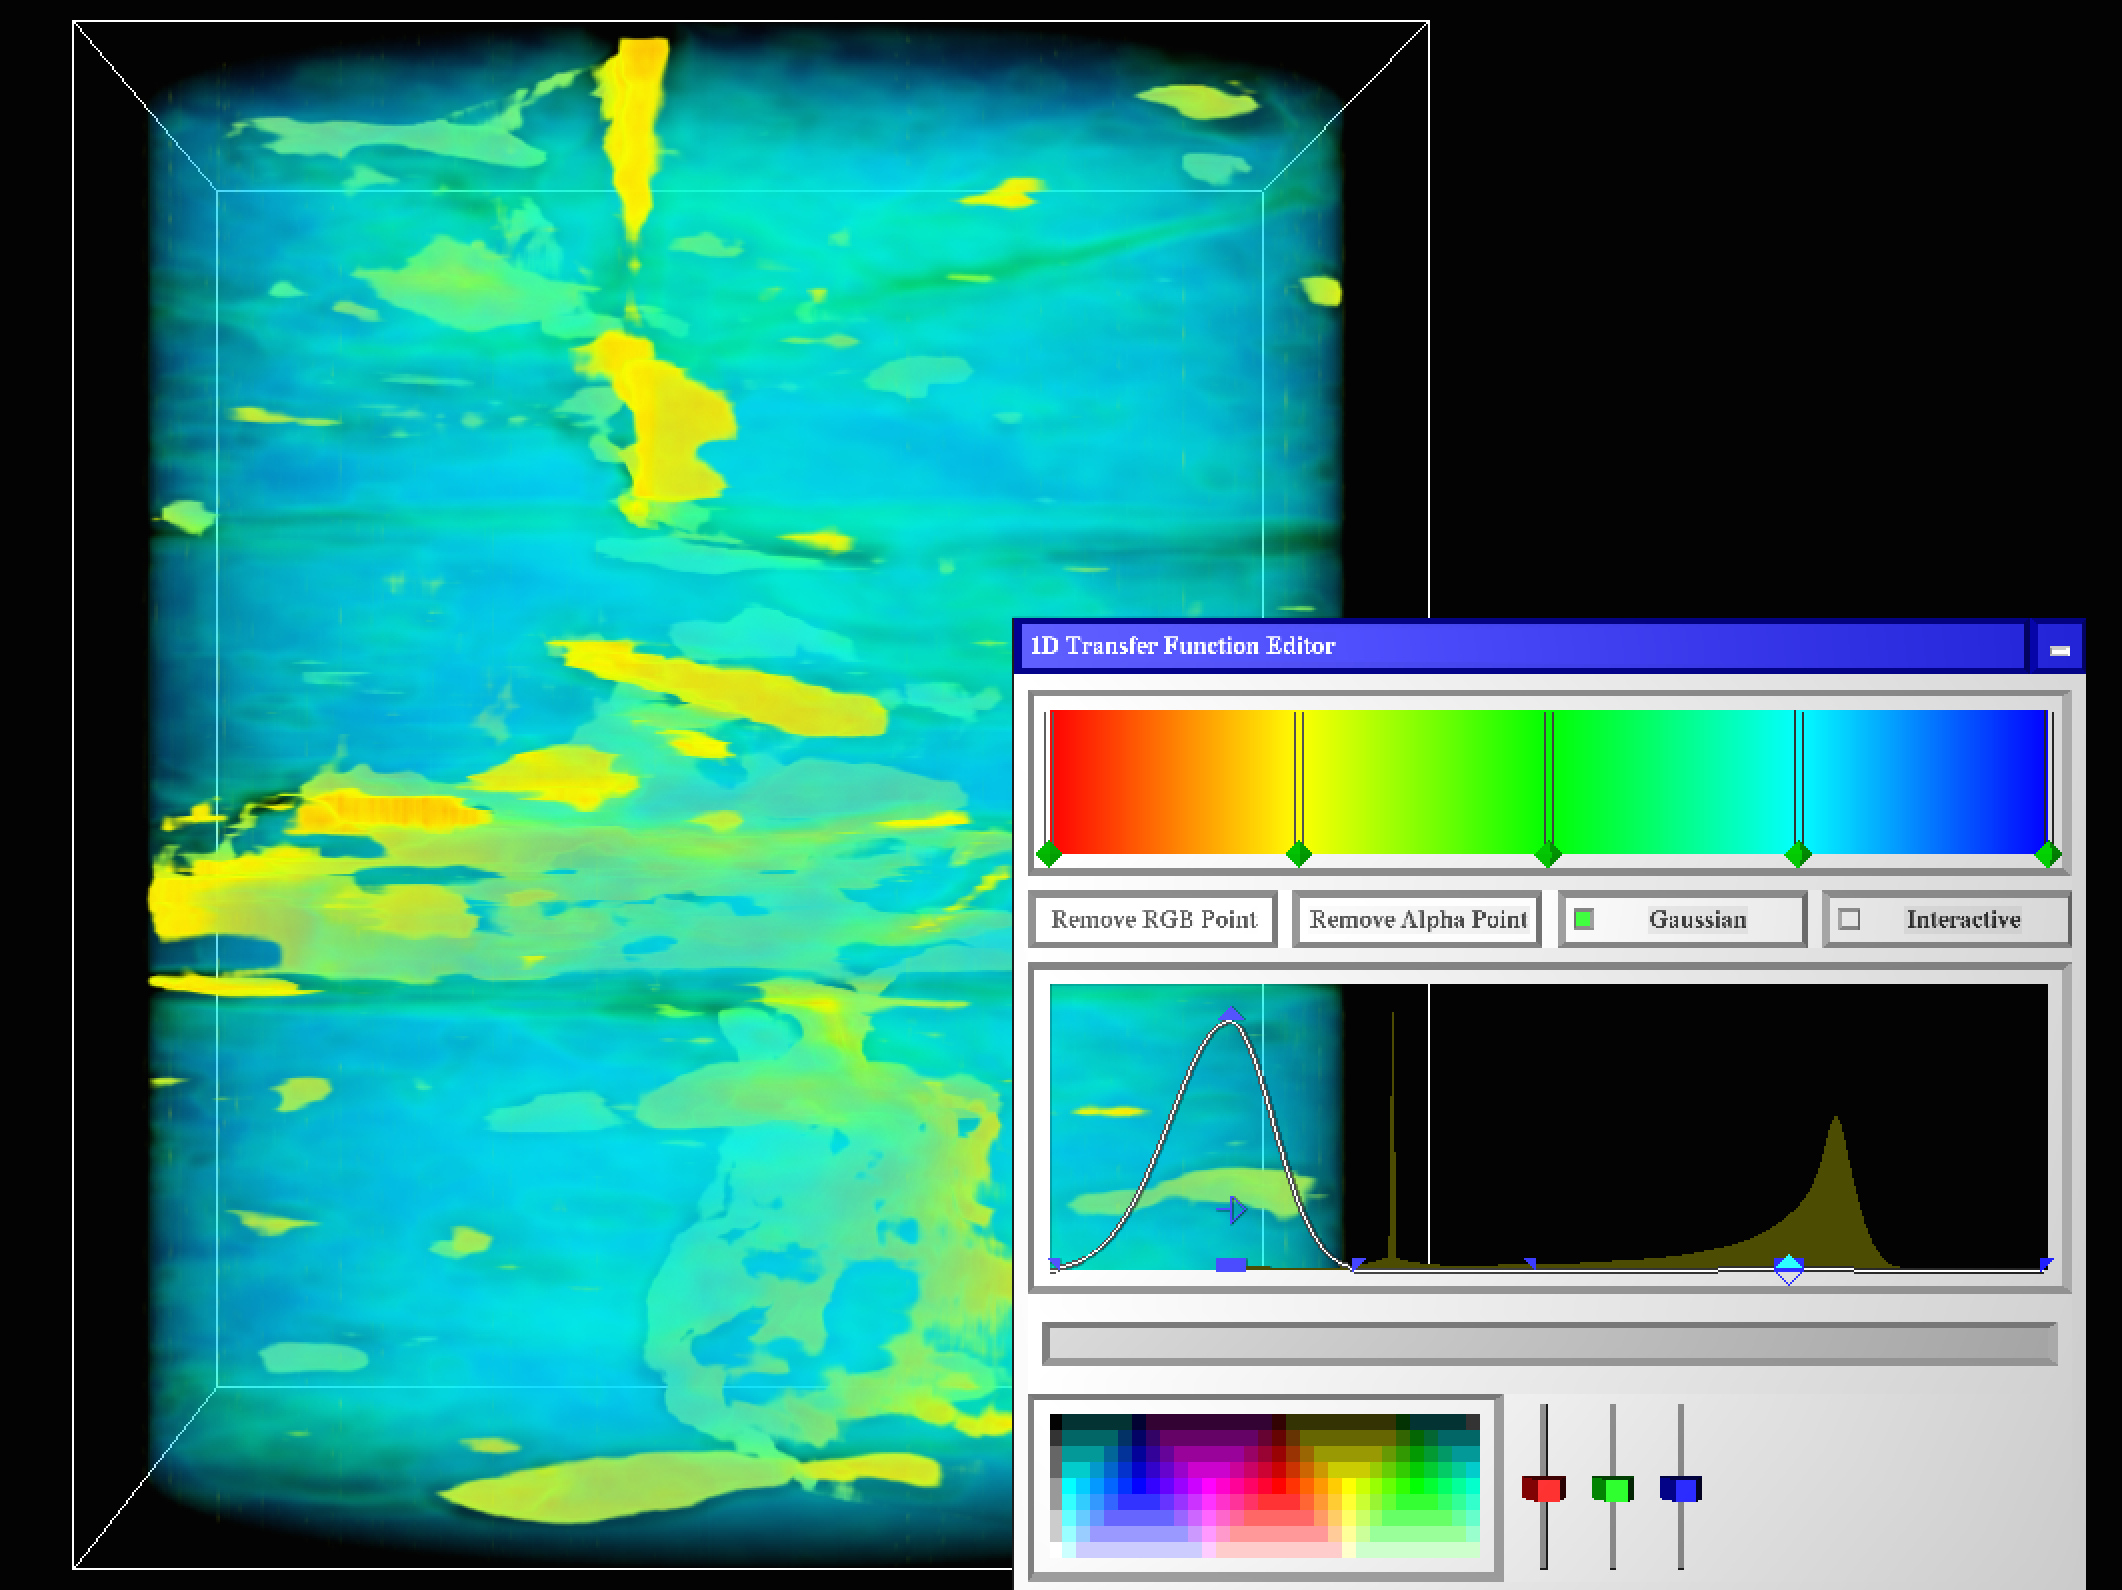
\includegraphics[width=3.5in]{images/rock-transferfunction.png}
 \caption{This is a digitized well ``rock" core. The yellow isosurfaces isolate the oil trapped within the shale rock.}
 \label{fig:volume}
\end{figure}

VolumeViewer~\cite{VolumeViewer} reads in and renders VTK ImageData (.vti) files that define structured points datasets.  The application instantiates a pipeline that allows volume rendering of the dataset. Several pre-defined \textit{Color Maps} help change mapping of scalar values to colors. A  \textit{Transfer Function Editor} allows varying color and opacity of the rendered volume.

Figure~\ref{fig:volume} depicts our implementation of a transfer function editor using Vrui's UI. In addition, we are leveraging the \texttt{vtkFlyingEdges3D} to display the oil isosurfaces in yellow while blending the results in the volume.

Widgets like Isosurfaces, Contours, Slice provide VTK level operations that can be carried out on the dataset. To circumvent possible interaction problems when dealing with large datasets, a low resolution mode is provided that down samples the dataset. This lets the end-user fulfill actions quickly that would otherwise take more time on the actual dataset, and then revert back to the actual size when done to visualize the output of performed actions at full scale.

\subsubsection{MooseViewer}

\begin{figure}[h!]
 \centering
 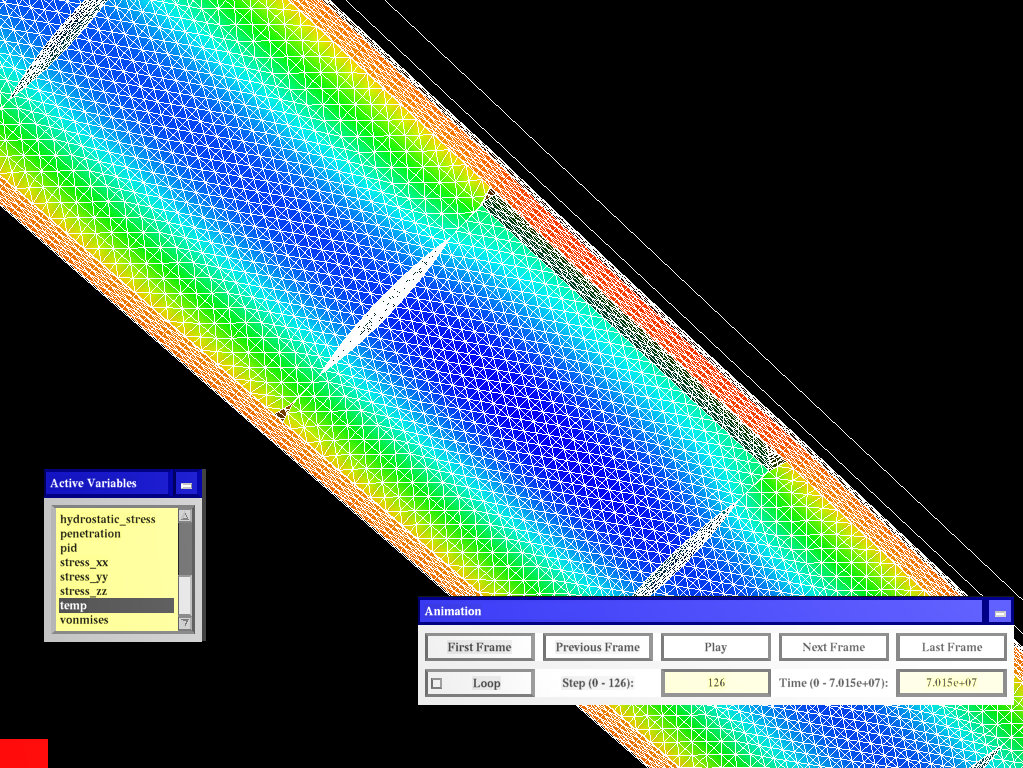
\includegraphics[width=3.5in]{images/fuelpin.png}
 \caption{A MOOSE Framework application BISON simulates a nuclear pin with missing cladding on one of the fuel pellets.}
 \label{fig:fuelpin}
\end{figure}

MooseViewer~\cite{MooseViewer} brings the ability of reading and displaying Moose framework~\cite{Gaston:2015, MooseFramework} ExodusII (.ex2, .e) files to immersive environments. The application uses \texttt{vtkExodusIIReader} to read geometry defined in ExodusII files as well as associated attributes (e.g. temperature, burnup, etc.). The application permits only user-selected variables to be loaded as data arrays, thus, reducing memory overhead. A \textit{Color By} sub-menu is dynamically populated with user-selected variables that maps the chosen variable scalars to colors using the \textit{Color Map} selected. An interesting feature of the application is animation of the dataset over time. The \textit{Animation Dialog} helps play through the time steps in the data file sequentially along with controls for looping over and stepping through the time steps.

We see, in Figure~\ref{fig:fuelpin}, surface geometry colored by the selected temperature attribute animated using the \textit{Animation Dialog}.

\subsection{OpenVR Implementation}

\subsection{Ply-file Example}

